\section*{Annexes}
\addcontentsline{toc}{section}{Annexes}

\subsubsection*{Annexe A: Planning de projet}

\subsubsection*{Annexe B: Dossier de fabrication}

\subsubsection*{Annexe C: Fiches techniques}

\iffalse

    \clearpage
    \vspace*{\fill}
    \begin{center}
        \begin{minipage}{.6\textwidth}
            \centerline{\Huge{Annexe A}}
        \end{minipage}
    \end{center}
    \vfill % equivalent to \vspace{\fill}
    \clearpage

    %Planning
    \includepdf[pages=-,rotateoversize]{Annexes/Planning.pdf}

    \clearpage
    \vspace*{\fill}
    \begin{center}
        \begin{minipage}{.6\textwidth}
            \centerline{\Huge{Annexe B}}
        \end{minipage}
    \end{center}
    \vfill % equivalent to \vspace{\fill}
    \clearpage

    %Mises en plans des pièces mécaniques
    \includepdf[pages={1-3},landscape=false]{Annexes/DossierFabrication}
    \includepdf[pages={4-14},landscape=true]{Annexes/DossierFabrication}
    \includepdf[pages={15-16},landscape=true,fitpaper]{Annexes/DossierFabrication}
    \includepdf[pages={17},landscape=true]{Annexes/DossierFabrication}

    \clearpage
    \vspace*{\fill}
    \begin{center}
        \begin{minipage}{.6\textwidth}
            \centerline{\Huge{Annexe C}}
        \end{minipage}
    \end{center}
    \vfill % equivalent to \vspace{\fill}
    \clearpage

    % Roulements
    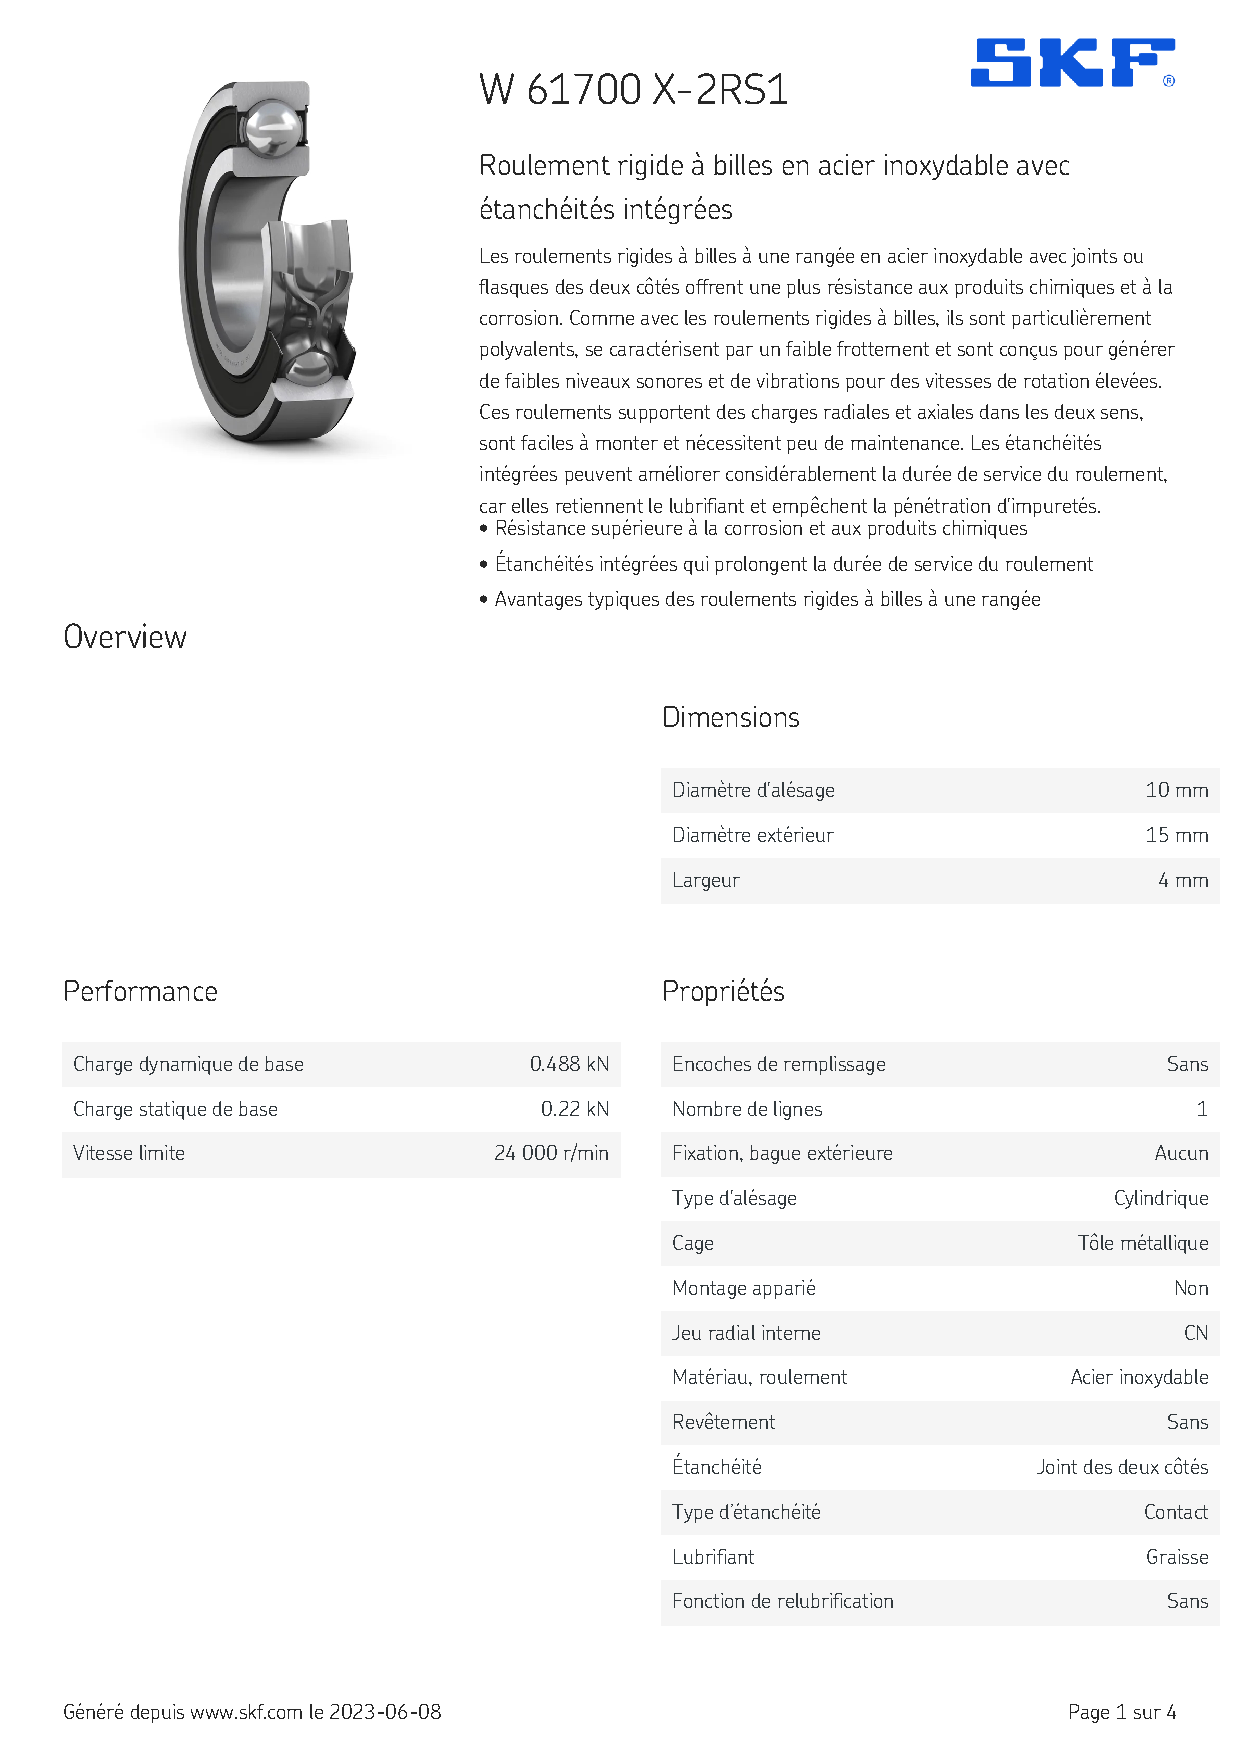
\includepdf[pages={1-2}]{Annexes/Roulement SKF W 61700 X-2RS1}

    % Moteur linéaire
    \includepdf[pages=-]{Annexes/Moteur lineaire}

\fi